\documentclass[10pt,a4paper]{article}
\usepackage[margin=2.2cm]{geometry}
\usepackage{fontspec}
\usepackage{kotex}
\setmainfont{Apple SD Gothic Neo}
\setsansfont{Apple SD Gothic Neo}
\usepackage{amsmath,amssymb}
\usepackage{graphicx}
\usepackage{booktabs}
\usepackage{caption}
\usepackage[dvipsnames]{xcolor}
\usepackage[colorlinks=true,linkcolor=MidnightBlue,citecolor=MidnightBlue,
            urlcolor=MidnightBlue]{hyperref}
\usepackage{titlesec}
\titleformat{\section}{\large\bfseries}{\thesection}{0.6em}{}
\titleformat{\subsection}{\normalsize\bfseries}{\thesubsection}{0.5em}{}
\captionsetup{font=small,labelfont=bf}
\setlength{\parskip}{0.35em}
\setlength{\parindent}{0pt}

\usepackage{mdframed}
\newmdenv[linewidth=0.4pt,linecolor=gray!60,backgroundcolor=gray!5,
          innertopmargin=6pt,innerbottommargin=6pt,skipabove=8pt,skipbelow=8pt]{claimbox}
\newcommand{\claim}[2]{\begin{claimbox}\textbf{주장.} #1\par\smallskip
  \textcolor{gray!70}{\textbf{반증 조건.} #2}\end{claimbox}}

\title{\bfseries 자를 부러뜨려 자를 통과하기\\[2pt]
\large 경계를 옮기니 효과가 7배 --- 잡음은 더}
\author{월드모델 실험실 · 노트 668}
\date{2026-08-06}
\begin{document}\maketitle

\section{한 줄}

같은 자료의 학습/유보 경계를 한 해 미뤘다. 팝업 학습 행이 $24 \to 68$ 이 되고 판
효과가 $+0.0016 \to \mathbf{+0.0115}$ (7.2배)로 올랐다. \textbf{그런데 위약도 같이
올라 부호가 뒤집혔고}($-0.0048 \to +0.0074$) 신호 몫은 오히려 줄었다. 사전등록
규칙대로 \textbf{기각}한다.

\section{왜 이걸 했나}

노트 663 이 열값(축 하나가 판에서 물어 가는 $\rho$)이 \textbf{학습 행 수에만}
달렸음을 확정했다 --- 빈 열은 정확히 $0.0000$ 이다. 노트 662 에서 지역 방문자 축은
신호 몫 $+0.0064$ 로 문턱 $0.0045$ 를 넘었는데 순효과는 $+0.0016$ 이라 채택이
아니었다. 차이를 먹는 것이 열값이므로 \textbf{학습 행을 늘리면 된다}.

노트 667 이 채굴 경로를 닫았다(수확률 2.2\%). 남은 길이 둘이었고 그중 싼 것이
\textbf{경계 이동}이다 --- \verb|T=2025.0| 을 \verb|2026.0| 으로 바꾸는 것뿐이다.
학습/유보가 이렇게 바뀐다: 팝업 $24/65 \to \mathbf{68/21}$ · 시장팝업
$123/126 \to 209/40$ · 채점 유보 합 $3{,}369 \to 1{,}287$. \textbf{11개 도메인이 다
살아남는다}(\verb|weights| 의 최소 20행 문턱을 다 넘는다).

측정 전에 배선 결함 하나를 고쳤다 --- \verb|lab/board.board()| 가
\verb|evaluate(T=T)| 는 넘기고 \verb|data.pooled(sc)| 는 \textbf{기본 2025} 로 가중을
만들고 있었다. 기본 $T$ 에서는 아무것도 안 바뀌므로 조용했다.

\section{문턱을 재서 정했다}

$0.0045$ 는 유보 3{,}369행에서 나온 표본 $2\sigma$ 다. 유보가 1{,}287행으로 줄면
그 문턱을 그대로 쓸 수 없다. 사전등록에 \textbf{어림 배율}
($\sqrt{3369/1287} \times 0.0045 = 0.0073$)과 \textbf{직접 재기} 둘을 같이 적었고,
도메인 안에서 행을 되뽑기($B{=}400$)해 짝 $\Delta\rho$ 의 SD 를 쟀다.

\begin{center}
되뽑기 SD $\mathbf{0.00624}$ $\to$ $2\sigma$ 문턱 $\mathbf{0.0125}$
\quad(어림 배율의 \textbf{1.7배})
\end{center}

\claim{\textbf{유보가 줄면 잡음이 $\sqrt{n}$ 보다 빨리 커진다.} 배율 어림이 1.7배
작게 나온 이유는 행 수만 줄지 않고 \textbf{도메인 가중이 소수 도메인으로 몰리기}
때문이다 --- 만화 유보 $258 \to 43$, 시장팝업 $126 \to 40$.}
{다른 $T$ 에서 되뽑기 SD 가 $\sqrt{n}$ 배율과 맞으면 이 주장은 특수한 경우다.
$T{=}2026$ 한 점에서만 쟀다는 것이 이 주장의 한계다.}

\section{쟀다 --- 네 팔}

\begin{center}
\begin{tabular}{lrrrrr}
\toprule
팔 & 판 & 차 & 양수 & 팝업 & 시장팝업 \\
\midrule
① 없이 & 0.4985 & --- & --- & --- & --- \\
② 팝업만 & 0.5011 & $+0.0026$ & 10/12 & $\mathbf{+0.0949}$ & $+0.0007$ \\
③ 팝업$+$시장 & 0.5100 & $\mathbf{+0.0115}$ & \textbf{12/12} & $+0.0591$ & $\mathbf{+0.3222}$ \\
④ 위약 & 0.5060 & $+0.0074$ & 12/12 & $+0.0409$ & $+0.1827$ \\
\bottomrule
\end{tabular}
\end{center}

배선을 매 팔에서 찍었다 --- 팝업 72행 · 시장팝업 238행. 열은 하나(\verb|vis_out|).

\begin{figure}[t]\centering
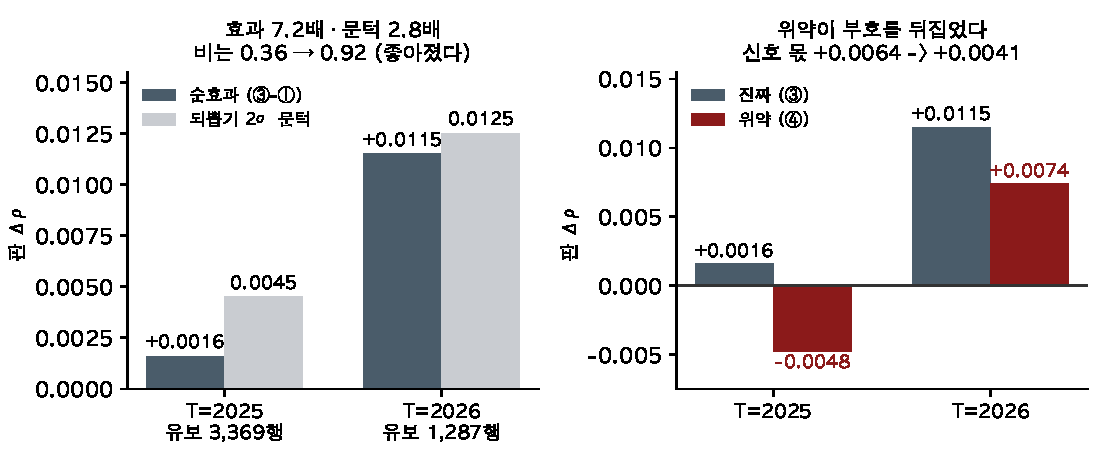
\includegraphics[width=0.99\textwidth]{figs/effectvsnoise.pdf}
\caption{왼쪽: 효과가 7.2배, 문턱이 2.8배 올랐으므로 \textbf{문턱 대비 비는
$0.36 \to 0.92$ 로 2.6배 좋아졌다.} 여기까지는 노트 663 의 법칙대로다. 오른쪽:
그런데 위약이 부호를 뒤집었다. \textbf{진짜와 위약이 같이 올랐으므로 오른 것은
신호가 아니다} --- 신호 몫 $+0.0064 \to +0.0041$(0.64배).}
\end{figure}

\section{왜 위약이 양수가 됐나 --- 한 도메인의 40행이다}

도메인 $\Delta\rho$ 에 유보 가중을 곱해 분해했다.

\begin{figure}[t]\centering
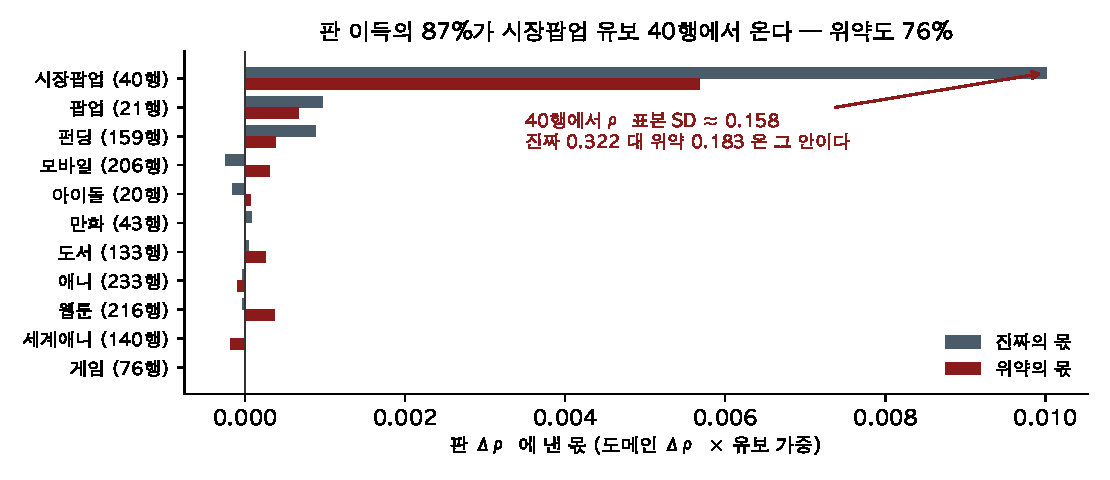
\includegraphics[width=0.99\textwidth]{figs/fortyrows.pdf}
\caption{시장팝업 유보 \textbf{40행}(가중 3.1\%)이 진짜의 \textbf{87\%} · 위약의
\textbf{76\%} 를 낸다. $+0.3222 \times 0.031 = +0.0100$ 이고 판 전체가 $+0.0115$ 다.}
\end{figure}

\claim{$T{=}2026$ 의 판 이득은 사실상 \textbf{시장팝업 유보 40행의 잡음}이다.
40행에서 $\rho$ 의 표본 SD 는 대략 $1/\sqrt{40} = 0.158$ 이므로 진짜 $0.322$ 와
위약 $0.183$ 의 차 $0.14$ 는 \textbf{1 SD 안}이다. \textbf{되뽑기 문턱이 정확히
그것을 값매김해서 두 팔을 다 떨어뜨렸다 --- 문턱이 제 일을 했다.}}
{시장팝업을 뺀 판에서 진짜와 위약의 차가 문턱을 넘으면 이 주장은 틀린다.
남은 열 도메인의 몫 합은 진짜 $+0.0015$ · 위약 $+0.0018$ 로 \emph{위약이 더 크다} ---
이 방향으로도 신호가 없다.}

\section{판정 --- 사전등록 규칙 ④}

사전등록에 이렇게 적었다: \emph{``신호 몫이 $T{=}2025$ 의 $+0.0064$ 보다
\textbf{작아지면} 경계 이동이 신호를 깎은 것이고 $\ldots$ 그러면 경계 이동을
되돌린다.''} 신호 몫이 $+0.0041$ 이므로 \textbf{규칙 ④ 가 발동한다.} 채택 규칙
①②(신호 몫과 순효과가 둘 다 문턱을 넘어야 한다)도 둘 다 미달이다. \textbf{경계는
2025 로 둔다.}

\subsection*{내 예측은 절반만 맞았고, 틀린 절반이 더 중요하다}

예측은 ``순효과는 오르지만 문턱도 올라 반반''이었다. 순효과는 예측대로 크게 올랐고
문턱 대비 비까지 좋아졌다. \textbf{예측하지 못한 것은 위약의 부호 반전}이고, 판정은
거기서 갈렸다. 노트 335 의 조항이 왜 있는지가 이 한 줄에 들어 있다 ---
\emph{위약이 진짜보다 나쁘지 않으면 신호가 아니라 차원 비용이다.}

\section{그래서 길이 하나 줄었다}

\claim{\textbf{같은 행을 학습으로 옮기는 것은 자를 부러뜨려 자를 통과하는 일이다.}
학습 행이 늘어 도메인 $\rho$ 는 실제로 크게 올랐다(팝업 $+0.009 \to +0.0949$).
그런데 그 행이 유보에서 빠지므로 \textbf{판정 분해능이 같이 무너진다.} 행을 늘리는
두 길 중 \textbf{경계 이동은 닫힌다.}}
{홀드아웃을 잃지 않고 학습을 늘리는 방식(예: 시간 교차검증)이면 이 주장이 안 걸린다.
다만 이 판은 ``2025년 이후로 채점''이 자의 정의라 그 변경은 자를 바꾸는 것이고,
그러면 83개 노트의 판 수치와 못 견준다.}

남은 길은 \textbf{덮음을 다른 도메인으로 넓히기} 하나다. 방문자 축은 11개 도메인 판에서
\textbf{팝업 · 시장팝업 둘}에만 붙고 나머지 아홉이 열값을 낸다. 다음 실험은 판을 안
도는 계수다 --- \textbf{아이돌 도메인에 장소가 있나}(공연장 $\to$ 시군구), 덮음이
노트 661 의 게이트 ⑥($0.7$)을 넘나. 넘으면 세 도메인으로 넓혀 재고, 못 넘으면
\textbf{방문자 축의 천장이 두 도메인}임을 확정하고 (시간 $\times$ 대상) 다른 형태로 옮긴다.

\end{document}
